% This is the "Resting potential" to the Hodgkin-Huxley neuron model V2.0 book
% Last edited 2026.06.24

\iflatexml
\else
\minitoc
\fi

\ifx\magyar\undefined

\chapter{Resting Potential\label{ch:RestingPotential}}

\else

\chapter{Nyugalmi potenciál\label{ch:RestingPotential}}

\fi

Concerning the origin of the membrane's resting potential, we disagree that "the resting membrane potential is the result of the [low intensity]
passive flux of individual ion species through several
classes of resting channels"~\cite{PrinciplesNeuralScience:2013}.
This claim cannot be true: the flux is not passive
(to move the ions, energy required), furthermore,
no setpoint is defined, so some (low) current flows
due to the interplay of the electrostatically set setpoint
and the reversal potential of the ions inside and outside. 
The claim was already question-marked whether the membrane permeability is a primary property for the 
membrane potential generation, for a review, see~\cite{MembranePotentialPermeability:2024}.
That interpretation leads to causality issues~\cite{HH_Potential_Controversies_2017}. 

% Physics of segmented volumes
It was already guessed that the membrane's resting potential is of electrostatic origin~\cite{MembranePotentialAbsorption:2014,OriginMembranePotential:2018,Hodgkin-HuxleyAdsorption:2021,MembranePotentialPermeability:2024,MembranePotentialKeyFunction:2023}.
\index{resting potential}
When ions are confined in a closed volume,
they exist in a state of thermodynamic and electrical equilibrium.
However, those equilibrium states cannot be discussed independently.
\index{thermodynamic equilibrium}
\index{electrical equilibrium}
We must discuss them in a non-disciplinary way because the participating ions belong simultaneously to the disciplines of electricity and thermodynamics; furthermore, we must cross the borderline between discrete and continuous points of view 
of nature~\cite{VeghNon-ordinaryLaws:2025}.
Furthermore, the features of living matter may change when measured 
in physics laboratories as usual.
When measuring them, we must consider that "the construction is different from anything we have yet tested in the physical laboratory"~\cite{Schrodinger:1992}.


\section[Thermodynamic field]{Deriving mebrane's "thermodynamic electrical field"\label{sec:Physics-ElectrolyteThermalField}}


In section~\ref{sec:Physics-ThermodynamicField}, we introduced the idea
of the "equivalent thermodynamic electrical field";
\index{equivalent thermodynamic electrical field}
now we calculate it for the case of neuron membrane 
as shown in .

\physicspanel{phys:EquivalentField_Membrane}
{The membrane's eqivalent electrical themodynamic field}
{
We assume that, in a balanced state, the concentrations on the two sides of the membrane are $C_{k}^{ext}$ and $C_{k}^{in}$, respectively; furthermore we assume that \[\frac{dC_{k}}{dz}\approx\frac{C_{k}^{ext}-C_{k}^{in}}{d}\]
To simplify the math writing, we neglect the change caused by considering 
the difference (maybe we should apply a near-unity factor); we use the larger concentration value instead. Using the constants and $T=300$, we can derive the "equivalent thermodynamic electrical field" across the membrane for the case of a permeable ion channel in the membrane

\begin{equation}
	E_{thermal}^{C_{k}}=-\frac{RT}{q*F}\frac{1}{C_{k}^{ext}}\frac{C_{k}^{ext}-C_{k}^{in}}{d} \approx -\frac{RT}{q*F}\frac{1}{d}
	\label{eq:NernstPlanckThermal1}
\end{equation}
\noindent
The equivalent thermodynamic electric field does not depend on concentration, but rather is linear in temperature and inversely proportional to membrane thickness (given in $nm$).
We provide the numerical values in \textbf{Numerics panel \ref{num:EquivalentField_Membrane}} for the case of ion channels in the membrane's wall.
}

\numericspanel{num:EquivalentField_Membrane}{Neuron's equivalent 
thermodynamic electrical field}
{
It is valid separately for all $C_k$
\begin{equation}
	E_{thermal}^{C_k}(d)=-2.585*10^{-2}\frac{1}{d}\quad \biggl[ \frac{V}{m} \biggr] \label{eq:NernstPlanckThermal2}
\end{equation}
Figure~\ref{fig:NernstPlanckThermalWidth} depicts the field's dependence on the membrane's width and how it compares
to the charge-generated electrical field.
The figure illustrates the setpoint(see section~\ref{Physics-ControlTheory}), the boundaries of the changes, and the interesting phenomena that occur within the shaded cross-section. The figure is an illustration, but its figures are not far from the true ones. For a $5\ nm$ membrane thickness, it results in $5.17*10^{6}\ \frac{V}{m}$, which compares well to the value provided by Eq.~(\ref{eq:ElectricGradient}).
(Notice that the membrane's thickness may change 
during the action potential, see~\cite{HeimburgPhysikOfNerves:2009}: 
the rush-in extra charge compresses the membrane. Similarly, the concentration of the electrolyte in proximity to the membrane 
also changes.) Correspondingly, by using that $U=E*d$, 
\begin{equation}
	U_{thermal}^{C_k}(5)=-25.85\quad \biggl[ {mV} \biggr] \label{eq:NernstPlanckThermal2A}
\end{equation}
}




\begin{figure}
\iflatexml
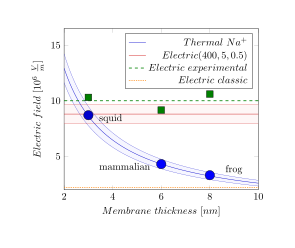
\includegraphics[width=\textwidth]{fig/NernstPlanckThermal.svg}
\else
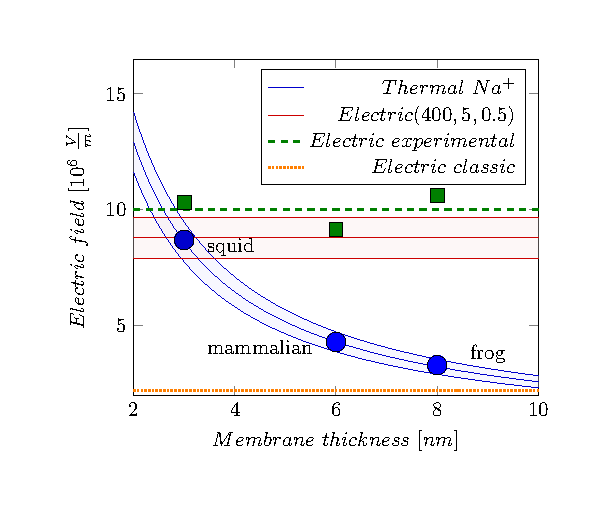
\includegraphics[width=.8\textwidth]{fig/NernstPlanckThermal.pdf}
\fi
	\caption{
		The thermodynamic "electrical field" depends on the membrane's thickness, see Eq.(\ref{eq:NernstPlanckThermal2}). %(the dotted line is to remember that $Na^+$ and $K^+$ gradients are of opposite direction).
The electrical gradient depends on the charged layer's concentration and thickness; see Eq.(\ref{eq:ElectricGradient}). The dots mark measured data shown in Table \ref{Tab:SummaryTable}.
		\label{fig:NernstPlanckThermalWidth}
	}
\end{figure}

\index{equivalent thermodynamic electrical field}



In simple words, the Nernst-Planck equation states that the changes in
concentrations of ions create changes in the electrical field (and
vice versa), and in a stationary state, they remain unchanged.
Notice that in the case of an ion mixture, a joint charge-generated electrical field exists, and they equal, per ion, the concentration-generated "electrical fields", see section~\ref{sec:Physiology-DerivingRestingPotential}.

In the steady state, in contrast with the case of an ion in the infinite space, some other forces also contribute to
the mentioned ones. To discuss how nature restores the steady state when a microscopic change occurs in a
balanced state of a biological solution, we write the well-known Nernst-Planck
equation (see Eq.(\ref{eq:NernstPlanck})) in a slightly extended form:
%
\begin{align}
	\underbrace{\bigl(-F_{constr}(z)\bigr)}_{Constraint} &= \underbrace{ e_{el}*E_{Gap}^{Total}(c,\Delta z)}_{Electrical} +\underbrace{e_{el}*E_{thermal}^{\textcolor{red}{C_k}}(d)}_{Thermodynamic}\\
	%\quad
	&\underbrace{\bigl(+F_{Transp}(z)\bigr)}_{Transport}\underbrace{\bigl(+F_{Invasion}(z)\bigr)}_{External} 
	%\quad\quad
	\label{eq:NernstPlanckExtended}
\end{align}
We multiplied the usual two terms by the elementary charge, so its terms are expressed as forces, plus we added an external force (its role is discussed below). Furthermore, changing one force triggers a corresponding counterforce and/or causes the ion to move in a viscous fluid. That is, the speed of the material transport gradually changes
as the steady state approached; furthermore, it is by orders of magnitude smaller than the speed of the interactions. 
When neuroscience teaches that "pumps that maintain
ion gradients \dots transport ions against their
electrical and chemical gradients"~\cite{PrinciplesNeuralScience:2013}, page 101, one shall ask \textit{what kind of force acts on the ion}, keeping in mind
E.~Schrödinger's opinion that not "any ‘new force’ or what not"~\cite{Schrodinger:1992} affects ions' motion.

An interesting option is when the counterforce combines two disciplines.
When $Na^+$ ions rush-in at the beginning into the membrane,
they produce simultaneously a huge electrical and thermodynamic gradient.
The repulsion among the ions creates a huge mechanical pressure
that presses the elastic membrane. The counterforce starts a mechanical 
shock wave (soliton)~\cite{SolitonPropagation:2005}, that is simultaneously
an electrical potential wave~\cite{VeghUnifiedCrossdisciplinaryModel:2026} that is measured as \gls{AP}. Only using  cross-disciplinary discussion (non-ordinary laws) enables understanding neuronal operation.  
That means when describing an ionic transfer process, \textit{we must not separate the electrical current from the mass transfer}: they happen simultaneously and mutually trigger each other. Notice that the thermodynamic term is ion-specific while the electrical term is not. To be entirely balanced, the system must be balanced to all elements. In this way, changing one concentration implicitly changes all other concentrations and the electrical field.

It was a colossal mistake to introduce equivalent circuits with their fixed-value voltage generators. It forces one to assume that the 
conductances of the players (membrane, synapses, \gls{AIS}) 
change 
without any reason and prevents understanding how the competition between thermodynamic and electrical processes governs neuronal operation.
It leads, among others, to attributing conductance change to membranes, which are simple isolators with no charge carriers that can implement
charge transfer, see section~\ref{sec:IonicCurrent}; this way
attributing the change of an electrical entity to the biological material.
This assumption neglects the driving force the mentioned forces provide. 
Instead, it attributes the magic ability to the ion channels that they
can change their transmission ability as the actual situation requires.

When discussing balanced states, no transport occurs, so the transport force cancels, and the mobility has no role. The counterforce adapts to the situation.
 That force may be a mechanical one:
the ions sitting on the surface of the membrane press the
surface due to the attractive force of ions, and the membrane mechanically provides the needed 
counterforce. 
If the boundary of the segments is not freely penetrable, the counterforce equals the difference between 
those two forces. In this way, no force acts on the ions; the two gradients persist. When the ions can move freely between the segments, they will move until they produce a concentration gradient (a thermodynamic force) for the given ionWhen neuroscience teaches that "pumps that maintain
ion gradients \dots transport ions against their
electrical and chemical gradients"~\cite{PrinciplesNeuralScience:2013}, page 101, one shall ask what kind of force acts on the ion, keeping in mind
E.~Schrödinger's opinion that not "any ‘new force’ or what not"~\cite{Schrodinger:1992} affects ions' motion.
 that counterbalances the electrical gradient (the electrical force)
and then the transport stops. A transport force is needed to reach the Stokes-Einstein speed (see Eq.(\ref{eq:StokesEinsteinSpeeddV})) in a viscous fluid.

We must not forget that initially, the Nernst-Planck equation described
a transfer process (i.e., a dynamic equation), assuming the same speed for mass and
charge transfers. We used it only to describe the balanced state (i.e., a static equation at zero speed) and added the term describing external (such as mechanical constraint) force that
may be involved; it affects the process, but it does not belong to either of the respective fields. Commonly known mechanical constraints appear in a non-conducting layer called the membrane, where that counterforce prevents ions from penetrating the membrane layers.
A membrane is a perfect isolator, i.e., no charge carriers exist
between its two surfaces, so it is senseless to introduce the notion of its conductance. (There may be ion channels that deliver ions built into the membrane, but it is a different subject.) The separation results from \textit{charge separation}, a mechanism distinct from \textit{polarization}, as typically described in most biology textbooks.
In the form we derived, the equation correctly describes 
the ion transfer, a current conveying ions with the speed controlled by the actual gradients, instead of assuming an ion current traveling 
with the apparent speed of electrical current in solids.


We must not forget that originally the Nernst-Planck equation described
a transfer process (i.e., a dynamic equation), assuming the same speed for mass and
charge transfers. We used it only to describe the balanced state (i.e., a static equation, at zero speed), and added the term describing external (such as mechanical constraint) force
may be involved; it affects the process, but it does not belong to either of the respective fields. Commonly known mechanical constraints are a non-conducting layer, called membrane, where that counterforce prevents ions from penetrating the membrane layers.
A membrane is a perfect isolator, i.e., no charge carriers exist
between its two surfaces. (There may be ion channels, that deliver ions, built into the membrane, as we discuss in section~\ref{sec:Demon-in-the-membrane}, but it is a different subject.) The current clearly results from \indexit{charge separation}; a mechanism distinct from \indexit{polarization} most biology textbook uses.
\index{polarization!membrane}
In the form we derived, the equation correctly describes 
the ion transfer, a current conveying ions with the speed controlled by the actual gradients, instead of assuming an ion current traveling 
with the apparent speed of electrical current in solids.



\section[Charge layers]{Charge layers in segment\label{sec:Physics-LayersInSegment}}

Figure~\href{https://www.ncbi.nlm.nih.gov/books/NBK26910/figure/A2034/?report=objectonly}
{the ionic basis of a membrane potential} shows and explains the case
introduced by separating the cell into two segments by a  finite-width membrane; although does not explain even qualitatively, \textit{why} the ions behave apparently against the laws of thermodynamics: the left and right sides of the figure are apparently identical. On the left side (the case of infinitely thin membrane), 
at an exact balance of charges on each side, the potential across the membrane is zero. 
We explain that the finite thickness will result in
a lack of balance (introduces inhomogeneity and creates a voltage and concentration gradient) proximal to the surfaces of the membrane, even if the concentrations on the two sides are the same. Changing the
bulk concentration or potential in one of the segments creates a corresponding
gradient across the separating membrane that increases the inhomogeneity proximal to the membrane.
The ions will experience an extra force due to the gradient,
but the mechanical counterforce of the membrane will keep them back in the segment. The \emph{concentration and
	potential, inseparably and having the same time course}, will change
across the two sides of the membrane just because of the gap's physical
features the membrane represents. 

We consider that the segment is composed of electrically conducting discs (the ions are free to move on the surface) and the charged discs' contribution to the 
electrical field at point $P$ (see Fig.~ \ref{fig:Physics-PointCharge}) can be calculated as known from the 
theory of electricity. Due to the symmetry in direction of $z$, in a homogenous solution, the resulting electrical field in the plane perpendicular to direction $z$ is zero: we have  contributions of the same size with opposite signs. 

Here we used the abstraction of an infinitely thin "charged sheet" and that there is a step-like
gradient in the electrical field in the gap. The physical reality is that the charge is represented by ions, which simultaneously represent a mass; furthermore, the thickness of the surface layer they form is by orders or magnitude thicker than the layer that the electrons form. In an equilibrium state, the forces due to the voltage and concentration gradients (see Eq.(\ref{eq:NernstPlanck})) must be counterbalanced by an external force.
%
An interference between science disciplines can also manifest here. We know at the same time that at the boundaries of electrolytes, different interfaces, including electrically neutral electrical double layers, can be formed by only partly known 
processes~\cite{ElectricDoubleLayer:2023}. The presence of those structures makes drawing quantitative conclusions hard.


\subsection[Classical condenser]{Simple conducting sheet (a classical condenser)\label{sec:Physics-SimpleSheet}}

When discussing the internal electrical operation of a neuron, first we consider a condenser that obeys 
laws of classical electricity and has 
the geometrical size of a biological neuron.
We apply the physics terms to that pseudo-biological object
and test whether the values we derive are consistent with physiological phenomena. A tiny (according to~\cite{JohnstonWuNeurophysiology:1995}, page~12, about~$2*10^{-3}$) portion of the positive ions leave their negative
counterions behind and form a thin positively charged ion layer on the surface of the membrane (of course, the same happens on the opposite side with negative ions). Experience shows, that -- also in biology -- two very thin (but not infinitely thin) layers of ions are formed on the two sides of the membrane, \href{https://www.ncbi.nlm.nih.gov/books/NBK26910/figure/A2034/?report=objectonly}{see the caption of figure (Fig.~11.22 in~\cite{MolecularBiology:2002})}:
"The ions that give rise to the membrane potential lie
in a thin ($< 1\ nm$) surface layer close to the membrane".
The two surfaces get covered by a sub-nanometer-thick
conducting layer, on the top of a $5~nm$ nanometer thick insulator. 
So, we model the cell with two finite-width "conductive sheet" layers.
\index{condenser}
These layers represent an electrical condenser (so we can calculate the internal electrical field between the plates) and they counterbalance each other's electrical field outside the condenser.
We may assume that the solid surface represents the needed
counterforce to keep the charges in rest.

One cannot expect geometrically plane surfaces: there are 
some biological objects of up to $1~nm$ size on the surface. So, we assume
a physical 'uniformly charged sheet' with an average thickness $\Delta z=0.5~nm$ on the surface.
For the sake of simplicity, we assume a step-like function
for the electrical field. It is zero in the segment outside 
the "conducting sheets" (the 'bulk' portions) as well as inside the sheets.  Between the sheets, it jumps to the value of the electrical field of a charged sheet with surface density $\sigma_A$ (see Eq.(\ref{eq:Physics-SurfaceChargeDensity})).
(In this picture we see that there is a jump in the value of the electrical field (and so: in the force acting on a charge)
in the two sides of the physical layer. Here we still assume that a mechanical counterforce due to surface's roughness keeps the charges in place inside the charged layer.)

We assume that all unbalanced (dissociated) ions are in the layer,
and the rest contains no dissociated ions, furthermore, that 
the ions' concentration is unchanged in the segment.
By assuming a~$0.5~nm$~thick layer on the surfaces of the membrane, our model delivers 
an electrical field (see Eq.(\ref{eq:Physics-ElectricFieldFromSigma}))
%
\begin{equation}
	E^{Gap}_{Classic}(c,\Delta z) = E_z(c,\Delta z) =
	4.45*10^3 * c  * \Delta z \quad 
	\biggl[ \frac{V}{m} \frac{1}{nm*mM} \biggr]
	\label{eq:Physics-EGapClassic}
\end{equation}
%
In the case of a $400~mM$ solution and a $0.5~nm$ 'thin physical layer'
it evaluates to an electrical field 
\[E^{Gap}_{Classic}(400,0.5)=0.11*10^7 \bigl[\frac{V}{m}\bigr]\]
and at a $5\ nm$ membrane thickness the voltage across the plates becomes
%
\begin{equation}
	U^{Gap}_{Classic}(400,0.5,5)= 
	2*E^{Gap}_{Classic}(400,0.5)*10^{-3}* d  = 10.84\ \bigl[mV\bigr]
\end{equation}
\noindent
The number of uncompensated ions needed for the cell, using the method in~\cite{JohnstonWuNeurophysiology:1995}, is $0.88*10^7$.
Remarkably, the calculated values are about by a factor of $5$ lower than 
the experimentally derived values.
"An
electrical potential difference about $50-100\ mV$ ... exists across
a plasma membrane only about $5\ nm$ thick, so that the resulting
voltage gradient is about $100,000\ V/cm$"~\cite{MolecularBiology:2002}. "The number of uncompensated ions needed for the cell is $4.7*10^7$"~\cite{JohnstonWuNeurophysiology:1995}. 
%
We are in the right order of magnitude but we arbitrarily assumed a layer thickness, a non-dielectrical medium. Furthermore, given that the charges are distributed uniformly in the layer, the electrical field changes linearly between the two sides of the conducting sheet. 
The deviation from the experienced values suggests that the dipoles' presence in the electrolyte bulk significantly changes the achievable electrical field and potential across the plates. Our simple model seems to be
a strong oversimplification.

\begin{figure}
	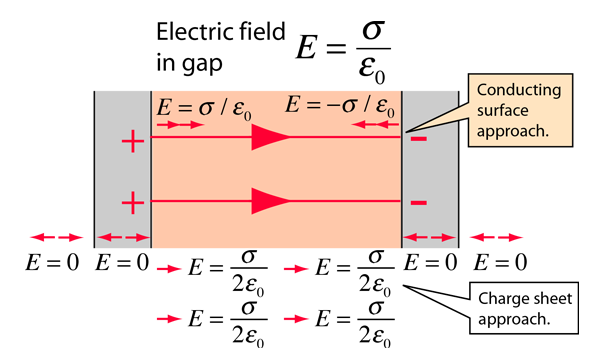
\includegraphics[width=.85\textwidth]{fig/eplat4.png}
	
	\caption{The oppositely charged parallel surfaces of the membrane are treated like  conducting plates (infinite planes, neglecting fringing),
then Gauss' law can be used to calculate the electrical field between the plates. Presuming the plates to be at equilibrium with zero electrical field inside the conductors, then the result from a charged conducting surface can be used.\label{fig:Physics-Capacitor}}
\end{figure}


If the 
distance between the plates is finite, the resulting electrical field will differ from zero. 
With such a model, a usual parallel plate condenser can be derived, as shown in Fig.~\ref{fig:Physics-Capacitor}.
We have two charged disks (infinite conducting sheets), and 
an insulator layer between them. In the classical picture, 
the opposite charges'amount on the two plates must be the same.
As shown, a constant electrical field is present inside the membrane (across the plates of the condenser) and zero electrical field inside the parallel conducting plates, as well as outside the condenser.
In this ideal picture, the charges are aligned on the border of two (infinitely thin) conducting layers and cannot move.
Anyhow, the attractive force between the opposite charges on the plates 
keeps them fixed in direction of $z$. The repulsive force
between the charges with the same sign keeps their surface density in the $(x,y)$ plane uniform: the infinitely thin plates are equipotential.
% (as discussed in section~\ref{sec:Physics-ThermoElectroDynamics}.
The strong electrostatic force can produce an enormous acceleration for the individual ions, but the thermodynamic gradient can only change with a several orders of magnitude lower speed, allowing measurable changes in the current intensity on the surface).
This picture is valid for the equilibrium state of charges, infinitely small non-dissociating charge carriers and perfectly smooth surfaces. 

Figure~\ref{fig:The-membrane's-extra-gradient} (the blue diagram lines) show the electrical field around the neuronal membrane.
In this picture we see that there is a jump in the value of the electrical field (and so: in the force acting on a charge)
in the two sides of the physical layer and we assume that the physical layer somehow emulates the well-defined boundary
on the side opposite to that proximal to the membrane. 




\subsection[Electrical field]{Electrical field in a two-segment electrolyte\label{sec:Physics-ElectricalField}}

Fig.~\ref{fig:The-membrane's-extra-gradient}
displays how the function shapes of electrical field
change in the function of the distance from the membrane. 
As discussed, the physical distance between two two segments
with electrical charge causes a charge condensation on the
surface of the separating membrane. In the case of classic condenser, this primary charge density 
is abstracted as an infinitely thin layer of charges (electrons)
on an ideally plain layer, and the rest of the volume is abstracted
that no charge carrier is included. This case is perfectly described by the classic electricity theory.
In the case of electrolytes, the separating membrane's surface is not ideal,
furthermore the electrostatic force can press some biological objects
to the surface, so we must assume that the primary charge forms a
uniformly charged layer with finite thickness on the surface.
In the uniformly charged layer the electrical field is a linear function
of the distance from the surface.
The presence of dielectrical molecules in the rest of the volume creates secondary (virtual) dipole charges, that contribute to the electrical field, as shown.
The two fields join to each other at the boundary
of the charged layer.
The electrical field on the surface of the membrane is the sum of those two fields.
The opposite charges on the other plate generate another electrical field in the opposite direction.

As shown in the figure, the field steeply rises near to the membrane.
At the membrane surface, it reaches its maximum value; on both sides of the membrane. Inside the membrane, there are no charges, so the field remains contant, for both types of condensers.
Notice that the classic condenser can be considered 
as the abstraction of the real condenser to the case of zero dielectricity.


The electrical field acts on the ions, but there may be present a mechanical counterforce,
plus a thermodynamic force aring from the difference of ions' concentrations.
(We just notice here that \textbf{\textit{the electrical driving force does not depend on the chemical type of the ions, but the thermodynamic force does}}.
The mechanical counterforce is adaptive, per ion, so it can keep different types of ions in rest.)
If there are 'holes' (ion channels) in the membrane, there is
no mechanical counterforce, so the ions could move under the effect of the difference between the electrical and thermodynamic forces.
The latter depends on the chemical nature of the ions, so it natively
provides selectivity: the resulting forces are different for ions of different types. The usual "downhill" method of explanation must
be corrected: the \textit{resulting potential} instead of the \textit{electrical potential} defines how the ions move.

The figure shows two ions (green and red) at the axis of the ion channel in two positions (the empty circles along the axis of the ion channel), at the beginning and end of a movement, when the ion channel is open.
On the diagram lines, filled circles show the electrical fields 
on the diagram lines at the position of the ions.

In the charged layer the ion \textit{density} is constant, that is the thermodynamic force is zero while the electrical force decreases with
the distance from the membrane's surface

If the channel opened, the mechanical counterforce cancels,
the ions will move under the effect of the resulting force,
that comprises not only the thermodynamic and electrical forces,
but also the force to move the ion with the Stokes-Einstein speed.
In the position at the entrance of the ion channel (see the red ions), if the channel is open, the large thermodynamic and electrical forces 'push' the ions into the channel. Here the concentration gradient quickly cancels, but the huge potential gradient will accelerate it toward the other segment. After passing the membrane with a high speed, the ion faces a quickly decreasing field, and its speed quickly decreases. The leave of ions changes both concentration and charge density in the vicinity

In the position farther from the membrane's surface (see the green ions) the ions must travel 'uphill'; that is, they cannot travel instantly toward the membrane.
They must wait until the gradient change caused by the ions pushed into the gap reaches their position.
As the figure shows, the ions quickly move out from the region with
high charge density and very slowly refill that region with ions from the region farther from the membrane.
This speed difference results in a quick change in the local electrical field.
In the region of the other plate, the ions decrease the (opposite)
local potential. As the result, there are less ions ready to travel
on the one side, and the potential difference continuously decreases
on the other, so the flow of ions stops: the ion channel shuts itself down (and, on both sides, starts to regenerate the potential as it was 
before the channel's cap was removed).
That is, the ion channel is opened by a slow mechanical cap,
but it is closed by a fast electrical shutter. While the potential
self-closes the channel, the electrical fields on  the two sides of the membrane have to relax: the ions and dipoles have time to change their
position and even their polarization and ionization state.
The local gradients will rearrange concentration and electrical field in the segment.


As depicted, in the two regions, there is a significant difference
in the value of the effective force acting on the ions (they are using $E_{accelerate}$ and $E_{assist}$, so they
produce different Stokes-Einstein speeds (see Eq.~(\ref{eq:StokesSpeed})). Based on those speeds,
one can introduce "fast" and "slow" ions
and correspondingly, speak about \emph{'slow' and 'fast' currents}
that the ions represent at a macroscopic level.
The corresponding
speeds also differ by orders of magnitudes. For this study, we
assume the diffusion, potential-assisted and potential-accelerated
speeds, in $m/s$ to be $10^{-4}$, $10^{-1}$ (also inside neurons~\cite{ActionPotentialGenerationNatrium:2008}),
\index{speed!diffusion}
\index{speed!potential-assisted}
\index{speed!potential-accelerated}
$10^{+3}$, respectively (used only to estimate the order of magnitude
of some respective operating times). When staging, we assume the greater
of the mixing speeds as 'infinitely large' and omit the time that
the process needs, while discussing how the slower process proceeds.


\begin{figure}
\iflatexml
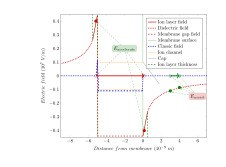
\includegraphics[width=.85\textwidth]{fig/DielectricMembrane.svg}
\else
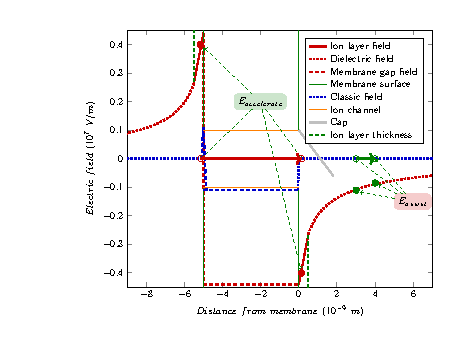
\includegraphics[width=.85\textwidth]{fig/DielectricMembrane.pdf}
\fi
\caption{The neuronal membrane's \emph{electrical field} in the function
of the distance from the membrane's surface and the bulk potential.
The thickness of the atomic layers proximal to membrane's surfaces
are also shown.\label{fig:The-membrane's-extra-gradient}}
\end{figure}

We are in line with the estimation given in~\cite{MolecularBiology:2002}
that in the case of resting potential, the scale of the gradient that
accelerates the ions across the ion channel is calibrated approximately
as $kV/cm$. Recall that we are still speaking about the resting state
and only about the extra gradient evoked by the finite-width membrane.
We are at the boundaries of the macroscopic and microscopic worlds.
We derived our integrand from the picture of discrete charges but
integrated it into the picture of continuous charge distribution. We assume an
\hypertarget{atomic_layer}
{atomic layer}
\index{layer!atomic}
(a skin) on the surface. However, the layer itself can also be modeled
as having just a few ions under their mutual repulsion on the surface
or a few atomic layers on top of each other, depending on the concentration
and voltage in the bulk on the two sides. (The diagram line is valid
in the plane crossing the membrane and the ion channel.) 


We assumed that the membrane's width is $5\ nm$. An ion channel is
depicted in the middle of the figure with a diameter of about $1\ nm$.
Furthermore, we assume that the ion's size and, correspondingly, the
thickness of the atomic layer in the electrolyte on the surface of
the membrane is about $0.1\ nm$. For comparison, recall that the
size of the tip of the clamp pipette is in the range of $1,000\ nm$
and the size of the soma in the range of $10,000\ nm$. 

Our results align with the observation (see caption of 11.22 in~\cite{MolecularBiology:2002}:
"A small flow of ions carries sufficient charge to cause a large change in the membrane potential.
The ions that give rise to the membrane potential lie in a thin ($< 1\ nm$) surface layer close to the membrane".
See the dotted line in Fig.~\ref{fig:The-membrane's-extra-gradient}; notice that the x-scale on the figure spans $1\ nm$ only.
\index{ion skin}
The amount of unbalanced ions is in the range of $10^7$,
and so is the amount of rush-in ions. In addition, those 
ions on the high-concentration side rush-in to the 
low-concentration side and cause the large change in the 
membrane potential. Their absolute amount is small compared to the total number of ions in the cell,
but it is significant compared to the number of unbalanced ions.


\subsection{Membranes with ions channels\label{sec:Physics-MembranesWithChannels}}

The attraction between the ions in the two skin layers
prevents the ions in the layers on the two sides from diffusing into/from
the bulk without a current drain in the layer for an extended period.
This steady state results from the interplay of the concentration
and the potential described by Eq.~(\ref{eq:NernstPlanck}). The gradients
change gradually within the segments and drop suddenly across the membrane.
No current can flow through the membrane; there is no leakage current.
\index{leakage current}

\index{voltage gradient}


Here, we
assume that no ion channels are in the excellently isolating wall
(ion channels would mean a current drain and, therefore, a voltage
drop). 

\section{Goldman-Hodgkin-Katz potential\label{sec:Physics-Goldman-Hodgkin-Katz}}


It was already stated, based on experimental evidence, that "the membrane permeability to the ions has nothing to do with the potential generation and the ions adsorption on the membrane surface generates the membrane potential", for a review see~\cite{MembranePotentialPermeability:2024}.
The idea itself is nonsense: in a balanced state, no ion transport happens, so even without permeability, the balanced state persists;  the resting potential has nothing to do with either ions' mobility or permeability nor with ion absorption~\cite{Hodgkin-HuxleyAdsorption:2021}.
Furthermore, there is no idea in \gls{GHK} about whether the 'setpoint' (why that specific concentration or potential difference) is present and why the same potential is reset after rough perturbations such as issuing an \gls{AP} or replicating a cell.
The causality is reversed: the potential is a static concept which is set electrically, and
the two gradients form the experienced concentrations and potentials from the available solvent molecules.
For the time course of forming the gradients, mobility and permeability play a role, but not in determining the concentrations or the resting potential.


In our clear physical picture, the thermodynamic forces on the one side
and on the other side of the membrane are summed. They counterbalance each other; furthermore, jointly the effect of the neuronal condenser, see  Fig.~\ref{fig:RestingPotential3}.
As we emphasized, the concentration gradients are ion-specific.
Furthermore, as we discussed in connection with Eq.(\ref{eq:Nernst1}), the \hyperlink{NernstLaw}{Nernst equation} comprises a per-ion indefinite constant (a potential difference).
To calculate a linear combination of terms comprising an arbitrary constant is nonsense,
and so is adding absolute concentrations on the different sides of the membrane, or changing the base of the logarithm used in a calculation to match
the experimental value. It is not more than number magic. The potential is described by coupled equations as discussed in connection with Eq.~(\ref{eq:coupling}).

The $Ca^{2+}$ ions do not fit into the \gls{GHK} picture. 
One of the reasons why \gls{GHK} cannot be good is that $[Ca^{2+}]$
is omitted. Biologically, it is hard to believe that $Ca^{2+}$ does not participate in the game of life (especially since biology sees the need for $Ca^{2+}$ pumps). Physically, one concentration alone on one side of the membrane cannot keep balance; as the different ion exchange processes, Table~\ref{Tab:SummaryTable} and Fig.~\ref{fig:RestingPotential3} show.
When adding a new ion to the solution, the sum concentration
increases, and so the electrical force increases, forcing the previous 
elements to find new concentrations on both sides.
The appearance of a new chemical element indirectly changes the concentrations of the others (a good example is the role of the negligible amount of $Ca^{2+}$).

%\subsection[Goldman-Hodgkin-Katz potential]{GHK potential\label{sec:Physics-RestingGHK}}
In the light of our findings, we must reconsider a few key conceptions. We derived (see Eq.(\ref{eq:UGapTotal400})) that the gap voltage depends on the thickness of the membrane and the overall concentration. 
Furthermore, we demonstrated that the gap voltage is equivalent to the resting potential (correctly: potential difference) and is independent of ion mobility or ion composition in the solution.
Derived values, such as the Goldman-Hodgkin-Katz potential, should be rethought. The idea is nonsense: in a balanced state, no ion transport happens, so even without permeability, the balanced state persists;  as experiments proved, the resting potential has nothing to do with either ions' mobility or permeability nor with ion absorption~\cite{Hodgkin-HuxleyAdsorption:2021}.
The causality is reversed: the potential is a static notion and is set electrically, and
the two gradients form the experienced concentrations from the available solvent molecules.
For the time course of forming the gradients and maintaining the balance, mobility and permeability play a role but not in determining the concentrations or the resting potential.

The $Ca^{2+}$ ions do not fit into the GHK picture. However (see our Table~\ref{Tab:SummaryTable}), it provides a thermodynamic contribution in the
same order of magnitude as the charge separation by the membrane. If we add
the potential due to $Ca^{2+}$, we arrive at the correct result that the total balance of the thermodynamic contributions equals zero, that is, the resting potential is zero. The electrical potential contribution is an additional term, resulting in the resting potential.


When adding a new ion to the solution, the sum concentration
increases, and so the electrical force increases, forcing the previous 
elements to find new concentrations on both sides.
The appearance of a new chemical element indirectly changes the concentrations of the others (a good example is the role of the negligible amount of $Ca^{2+}$). No linear summing or similar assumptions can be made. The potential is described by coupled equations as discussed in connection with Eq.(\ref{eq:coupling}).
As we discussed in connection with Eq.(\ref{eq:Nernst1}), the integral form of the Nernst equation implies an undetermined additive constant. To calculate 
a linear combination of terms comprising an arbitrary constant is nonsense,
and so is changing the base of the logarithm used in a calculation to match
the experimental value.

\section{Moving in the membrane's potential\label{sec:Physics-MovingPotential}}


In Fig.~\ref{fig:The-membrane's-extra-gradient},
an ion channel is
depicted in the middle of the figure with a diameter of about $3\ nm$ for visibility.
Furthermore, we assume that the ion's size and, correspondingly, the
thickness of the atomic layer in the electrolyte on the surface of
the membrane is about $0.1\ nm$ (although with their electrical double layers, they can also reach the size of $1\ nm$). For comparison, recall that the
size of the tip of the clamp pipette is in the range of $1,000\ nm$
and the size of the soma in the range of $10,000\ nm$. 


\subsection{Passing through ion channels\label{sec:Physics-PassingIonChannels}}
Figure~\ref{fig:The-membrane's-extra-gradient} also hints at how ions can move in the proximity of the membrane. On the left side, the electrical field increases toward the membrane, so the ions cannot move in that direction without an initial force being applied. The case is the same on the right side, because the charge is the opposite.
An ion must gain energy to get closer to the membrane, which means, at the same time, higher potential energy.
This situation explains why the ions do not diffuse into the bulk region.
At their present positions, the counterforces by the membrane (and the dipole layer on it)
balance the attraction from the opposite side.  The ion channels
can work in continuous mode (the "resting ion channels") and
impulse mode (gated by "caps" on the channels, in transient mode).

Notice that the resulting electrical field cannot accelerate an ion 
except when the ion is at the beginning of the open ion channel across the membrane. Here, the mechanical counterforce is missing, and the field drops to the value generated by the 
condenser inside the plates. Here, a vast electrical field accelerates the ions to a high speed (although a force needed to move against the viscosity decreases the electrostatic acceleration). The empty red circles show
an ion that traverses through the channel.
The figure shows their electrical fields on the two sides, at the beginning and end of the channel. (On the right side, the electrical field is negative, but so is the charge of the ions.)

\subsection{Moving in the polarized electrolyte\label{sec:Physics-MovingPolarized}}

The electrical acceleration sharply decreases after leaving the ion channel (see the right side). As shown by the difference of the vertical positions of the filled red and green balls, the difference in the electrical field values is huge across the membrane ($E_{accelerate}$) and considerable inside the dielectric
electrolyte ($E_{assist}$) as shown by the difference in the electrical field values of the green balls. The field still accelerates, but significantly less intensely than the one in the gap. Suppose we assume that the ion quickly accelerates to its Stokes-Einstein speed. In that case, the travel speeds in
those space regions are proportional to the difference of the fields
in the shown positions and the reciprocals of their travel times. 

The passed ions decrease the concentration, and the electrical field
on the high-concentration side increases on the low-concentration side. Similarly, the gradients decrease and increase,
changing locally the gradients.
At the exit, the field continues to accelerate the ion. 
However, the increasing potential and concentration 
increasingly decelerate the passing ions, so they quickly brake them to the assisted speed. Then, the effect of the electrical field cancels, and the ions will move with their diffusion speed ("the ion stops").




\subsection{Ion selectivity\label{sec:Physics-IonSelectivity}}
As Eq.(\ref{eq:NernstPlanckExtended}) states, the electrolyte separated by a permeable membrane is balanced when the electrical and thermodynamic forces are equal. The $E_{thermal}^{C_k}(d)$ "electrical field" depends on the chemical quality of the ion; the electrical field does not. That means the resulting driving forces acting on the
different ions are different. While one ion experiences a resulting force and moves to the other segment, the other remains resting. Of course, the ions moving across the segments change the overall concentrations in both segments (and so the electrical field contribution), indirectly affecting the balanced state of the other ions. When a mixture of ions is present in the volume,
all ions feel a different driving force, and the solution as a whole will be balanced when the resulting forces for all chemical ions are balanced. The permanently open ion channels only passively participate in the process. The driving forces of the ions are different, and they produce, depending on the actual concentrations, the selectivity of the channels. 
\index{ion selectivity} 

When $Na^+$ ions rush into the intracellular layer, they roughly increase the overall concentration and the potential. All other ions, including $K^+$,  feel a driving force. The targeted membrane potential is set electrically, and the driving gradients may behave controversially during the transient period. The actual voltage gradient may temporarily direct the chemical gradient in opposite directions.
Phenomena such as 'over-relaxation', in this sense, similar to 'hyperpolarization', may happen.


However, the layer itself can also be modeled
as having just a few ions under their mutual repulsion on the surface
or a few atomic layers on top of each other, depending on the concentration
and voltage in the bulk on the two sides. (The voltage gradient diagram line validates
the plane crossing the membrane and the ion channel.) 


Our results align with the observation (see caption of Fig.~11.22 in~\cite{MolecularBiology:2002}).
\index{ion skin}
The amount of unbalanced ions is in the range of $10^7$,
and so is the amount of rush-in ions. In addition, those 
ions on the high-concentration side rush into the 
low-concentration side and cause a large change in the 
membrane potential. Their absolute amount is small compared to the total number of ions in the cell,
but it is significant compared to the number of unbalanced ions.




